\section{MPS algorithms}

This section and the following one, will introduce some different \Gls{TN} algorithms. The goal is to provide an intuitive explanation on how these algorithms work. For rigorous derivations and mathematical details, see e.g.\  \cite{Vanderstraeten2019}.

\subsection{Canonical form}

A translation invariant \Gls{MPS} is of the form \cref{mps:uni}. It can easily be seen that inserting $X X^{-1}$ on each bond doesn't change the contracted tensor. This is called a gauge transformation. Defining
\begin{equation}
    \begin{split}
        &A_l = \pepob{3}{2}{{
                    "-","-",
                    "",""}}{{
                    "-",
                    "",
                    "-"}}{{
                    4,4,4,
                    4,2,4}}  =X \pepob{3}{2}{{
                    "-","-",
                    "",""}}{{
                    "-",
                    "",
                    "-"}}{{
                    4,4,4,
                    4,0,4}} X^{-1} \\
        &A_r = \pepob{3}{2}{{
                    "-","-",
                    "",""}}{{
                    "-",
                    "",
                    "-"}}{{
                    4,4,4,
                    4,3,4}}=Y \pepob{3}{2}{{
                    "-","-",
                    "",""}}{{
                    "-",
                    "",
                    "-"}}{{
                    4,4,4,
                    4,0,4}} Y^{-1}
    \end{split}
\end{equation}
and
\begin{equation}
    \pepob{3}{2}{{
                "-","-",
                "",""}}{{
                "-",
                "-",
                "-"}}{{
                4,4,4,
                4,6,4}}  = X Y^{-1} = C ,
\end{equation}
\cref{mps:uni}  becomes
\begin{equation}
    \pepob{6}{2}{{
                "-","-", "-","-","-",
                "","","","",""}}{{
                "-",
                "",
                "",
                "-",
                "",
                "-"}}{{
                4,4,4,4,4,4,
                13,2,2,6,3,13}} .
\end{equation}
Define
\begin{equation}\label{algs:ACC}
    A_c = \pepob{3}{2}{{
                "-","-",
                "",""}}{{
                "-",
                "",
                "-"}}{{
                4,4,4,
                4,7,4}} = \pepob{4}{2}{{
                "-","-", "-",
                "","",""}}{{
                "-",
                "",
                "-",
                "-"}}{{
                4,4,4,4,
                4,2,6,4}} = \pepob{4}{2}{{
                "-","-", "-",
                "","",""}}{{
                "-",
                "-",
                "",
                "-"}}{{
                4,4,4,4,
                4,6,3,4}}.
\end{equation}
At the moment the matrices $X$ and $Y$ are not yet defined. To bring an \Gls{MPS} A in its canonical form, the following choice is made
\begin{subequations} \label{algs:mpsid}
    \begin{alignat}{3}
                     & \vcenter{ \hbox{ \pepob{3}{2}{{
                            "","",
                            "",""}}{{
                            "",
                            "",
                            "-"}}{{
                            4,2,4,
        4,2,4}} } }= &                                 & \vcenter{ \hbox{  \pepob{3}{2}{{
                            "","-",
                            "","-"}}{{
                            "",
                            "-",
                            "-"}}{{
                            4,4,4,
        4,4,4}} } }  &                                 & = I                              \\
                     & \vcenter{ \hbox{ \pepob{3}{2}{{
                            "","",
                            "",""}}{{
                            "-",
                            "",
                            ""}}{{
                            4,3,4,
        4,3,4}} } }= &                                 & \vcenter{ \hbox{  \pepob{3}{2}{{
                            "","-",
                            "","-"}}{{
                            "",
                            "-",
                            "-"}}{{
                            4,4,4,
        4,4,4}} } }  &                                 & = I .
    \end{alignat}
\end{subequations}
The tensors below are the conjugated version of the tensors above. There is still some freedom: a unitary gauge transformation can still be applied. With this choice, it is possible to bring $C$ in diagonal form. \cite{Vanderstraeten2019}

\subsection{Entropy}

The canonical form above is very convenient to calculate the entropy, which is given by
\begin{equation}
    S = -\sum_i \alpha_i^2 \log (\alpha_i^2 )
\end{equation}
where $\alpha_i$ are the singular values of $C$.

\subsection{Expectation value}\label{subsec:exp_val_1d}

One property of \Gls{MPS} is that expectation values can be calculated exactly. Suppose we have an operator $\hat{O}$ acting on a single site of the \Gls{MPS}: $\Braket{ \Psi |  \hat{O} | \Psi  }$
\begin{equation}
    \vcenter{\hbox{\pepob{5}{3}{{
                        "","", "","",
                        "-","-","-","-",
                        "","","","",}}{{
                        "-", "-",
                        "", "",
                        "", "",
                        "", "",
                        "-", "-",}}{{
                        13,2,7,3,13,
                        1,4,0,4,1,
                        13,2,7,3,13}} }}  =   \vcenter{\hbox{\pepob{5}{3}{{
                        "","", "","",
                        "-","-","-","-",
                        "","","","",}}{{
                        "-", "*-",
                        "", "",
                        "", "",
                        "", "",
                        "-", "-",}}{{
                        1,4,7,4,1,
                        1,4,0,4,1,
                        1,4,7,4,1}} }}
\end{equation}
where we made use of \cref{algs:mpsid}. Similar techniques allow for the calculation of correlation functions, energies, ...

\section{TN contraction}

Suppose we have an \Gls{MPO} $\hat{O}$ that represents a probability of encountering a given state: $ \hat{O} \ket{\Psi_i} = p_i \ket{\Psi_i} $. The average value of a local measurement X is given by $ \sum_i \Braket{ \Psi_i | \hat{X} \hat{O} | \Psi_i} = \Tr( \hat{X} \hat{O})$. This will be needed in \cref{subsec:statmech}. This section explains how to calculate this with \Glspl{TN} for infinite systems.

\subsection{1D problem}

The normalised expectation value of an observable $ \Braket{X}$ measuring several neighbouring sites is given by
\begin{equation}
    \Braket{X} = \frac{
        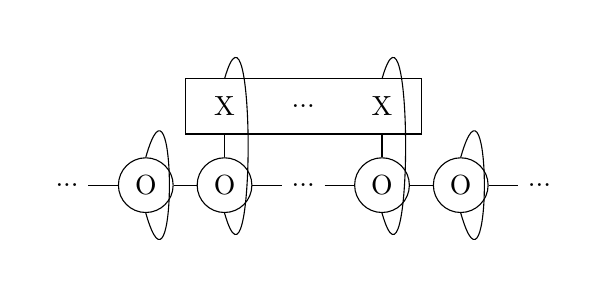
\begin{tikzpicture} [   ]
            \clip (-1.5,-1) rectangle (5.5,2);

            \node[] (N0) at (-1,0) {...};
            \node[circle, draw] (N1) at (0,0) {O};
            \node[circle, draw] (N2) at (1,0) {O};
            \node[circle, draw=none] (X2) at (1,1) {X};

            \node[] (N3) at (2 ,0) {...};
            \node[] (X3) at (2,1) {...};

            \draw  (0.5,0.65) rectangle (3.5,1.35);

            \node[circle, draw] (N4) at (3 ,0) {O};
            \node[circle, draw=none] (X4) at (3,1) {X};

            \node[circle, draw] (N5) at (4 ,0) {O};
            \node[] (N6) at (5 ,0) {...};

            \draw  (N0) -- (N1) ;

            \draw  (N1) -- (N2) ;
            \draw  (N2) -- (N3) ;
            \draw  (N3) -- (N4) ;
            \draw  (N4) -- (N5) ;
            \draw  (N5) -- (N6) ;

            %\draw  (X2) -- (X3) ;
            %\draw  (X3) -- (X4) ;

            \draw  (N2) -- (X2) ;
            \draw  (N4) -- (X4) ;

            \draw (X2.north)   .. controls +(0.4,1.4) and +(0.4,-1.4) .. (N2.south);
            \draw (X4.north)   .. controls +(0.4,1.4) and +(0.4,-1.4) .. (N4.south);

            \draw (N1.north)   .. controls +(0.4,1.4) and +(0.4,-1.4) .. (N1.south);
            \draw (N5.north)   ..  controls +(0.4,1.4) and +(0.4,-1.4)  .. (N5.south);

        \end{tikzpicture}
    }{
        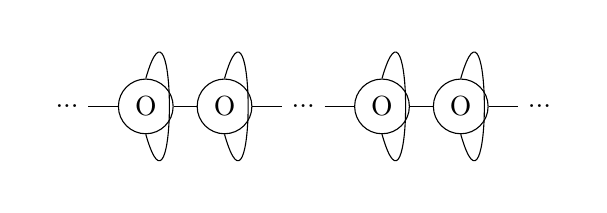
\begin{tikzpicture} [   ]

            \clip  (-1.5,-3) rectangle (5.5,-1);

            \node[] (O0) at (-1,-2) {...};
            \node[circle, draw] (O1) at (0,-2) {O};
            \node[circle, draw] (O2) at (1,-2) {O};

            \node[] (O3) at (2 ,-2) {...};
            \node[circle, draw] (O4) at (3 ,-2) {O};

            \node[circle, draw] (O5) at (4 ,-2) {O};
            \node[] (O6) at (5 ,-2) {...};

            \draw  (O0) -- (O1) ;

            \draw  (O1) -- (O2) ;
            \draw  (O2) -- (O3) ;
            \draw  (O3) -- (O4) ;
            \draw  (O4) -- (O5) ;
            \draw  (O5) -- (O6) ;

            \draw (O2.north)   .. controls +(0.4,1.4) and +(0.4,-1.4) .. (O2.south);
            \draw (O4.north)   .. controls +(0.4,1.4) and +(0.4,-1.4) .. (O4.south);

            \draw (O1.north)   .. controls +(0.4,1.4) and +(0.4,-1.4) .. (O1.south);
            \draw (O5.north)   ..  controls +(0.4,1.4) and +(0.4,-1.4)  .. (O5.south);
        \end{tikzpicture}
    }.
    \label{sm:expecatation_X}
\end{equation}
In the thermodynamic limit there are an infinite number of traced O to the left and the right. This can be solved by taking the left and right fixed points $Gl$ and $Gr$ of the traced \Gls{MPO} O corresponding to the largest eigenvector $\lambda$.
\begin{equation}\label{algs:exp}
    \begin{split}
        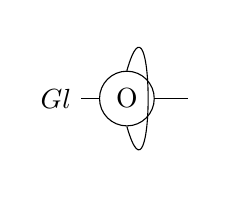
\begin{tikzpicture}[baseline={0cm-0.5*height("$=$")} , scale=0.9]
            \clip (-1.4,-1) rectangle (1,1);
            \node[] (N0) at (-1,0) {$Gl$};
            \node[] (N2) at (1,0) {};
            \node[circle, draw] (N1) at (0,0) {O};
            \draw  (N0) -- (N1) ;
            \draw  (N1) -- (N2) ;
            \draw (N1.north)   .. controls +(0.4,1.4) and +(0.4,-1.4) .. (N1.south);
        \end{tikzpicture}
        &= \lambda
        \begin{tikzpicture}[baseline={0cm-0.5*height("$=$")}, scale=0.9 ]
            \clip (-.4,0.5) rectangle (1,-0.5);
            \node[] (N2) at (1,0) {};
            \node[] (N1) at (0,0) {$Gl$};
            \draw  (N1) -- (N2) ;
        \end{tikzpicture} \\
        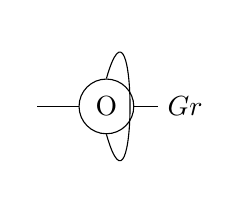
\begin{tikzpicture}[baseline={0cm-0.5*height("$=$")} ]
            \clip (-1,-1) rectangle (1.4,1);
            \node[] (N0) at (-1,0) {};
            \node[] (N2) at (1,0) {$Gr$};
            \node[circle, draw] (N1) at (0,0) {O};
            \draw  (N0) -- (N1) ;
            \draw  (N1) -- (N2) ;
            \draw (N1.north)   .. controls +(0.4,1.4) and +(0.4,-1.4) .. (N1.south);
        \end{tikzpicture}
        &= \lambda
        \begin{tikzpicture}[baseline={0cm-0.5*height("$=$")} ]
            \clip (0,-0.5) rectangle (1.4,0.5);
            \node[] (N2) at (1,0) {$Gl$};
            \node[] (N1) at (0,0) {};
            \draw  (N1) -- (N2) ;
        \end{tikzpicture}
    \end{split}
\end{equation}
Equation \cref{sm:expecatation_X} can now be easily calculated
\begin{equation}
    \Braket{X} = \frac{
        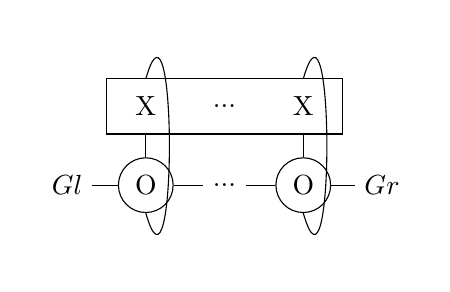
\begin{tikzpicture} [   ]
            \clip (-0.5,-1) rectangle (4.5,2);

            \node[] (N1) at (0,0) {$Gl$};
            \node[circle, draw] (N2) at (1,0) {O};
            \node[circle, draw=none] (X2) at (1,1) {X};

            \node[] (N3) at (2 ,0) {...};
            \node[] (X3) at (2,1) {...};

            \node[circle, draw] (N4) at (3 ,0) {O};
            \node[circle, draw=none] (X4) at (3,1) {X};

            \draw  (0.5,0.65) rectangle (3.5,1.35);

            \node[] (N5) at (4 ,0) {$Gr$};

            \draw  (N1) -- (N2) ;
            \draw  (N2) -- (N3) ;
            \draw  (N3) -- (N4) ;
            \draw  (N4) -- (N5) ;

            %\draw  (X2) -- (X3) ;
            %\draw  (X3) -- (X4) ;

            \draw  (N2) -- (X2) ;
            \draw  (N4) -- (X4) ;

            \draw (X2.north)   .. controls +(0.4,1.4) and +(0.4,-1.4) .. (N2.south);
            \draw (X4.north)   .. controls +(0.4,1.4) and +(0.4,-1.4) .. (N4.south);

        \end{tikzpicture}
    }{
        \lambda^n
        \begin{tikzpicture}[baseline={0cm-0.5*height("$=$")} ]
            \clip (-0.5,-0.5) rectangle (1.4,0.5);
            \node[] (N2) at (1,0) {$Gr$};
            \node[] (N1) at (0,0) {$Gr$};
            \draw  (N1) -- (N2) ;
        \end{tikzpicture}
    } .
    \label{sm:expecatation_X_2}
\end{equation}

\subsection{2D problem}
\Gls{PEPS} contraction concerns a similar problem, but in 2D. Here, instead of already applying operator X, the (one site) reduced density matrix $ \rho_{i,j}$ is computed:
\begin{equation}\label{algs:biggrid}
    \rho_{i,j} =\vcenter{ \hbox{ \pepob{7}{7}{{
                        "-","-", "-","-","-","-",
                        "",  "", "","","","",
                        "",  "", "","","","",
                        "",  "", "","","","",
                        "",  "", "","","","",
                        "",  "", "","","","",
                        "-", "-", "-","-","-","-",}}{{
                        "-","-", "-","-","-","-",
                        "","", "","","","",
                        "","", "","","","",
                        "","", "","","","",
                        "","", "","","","",
                        "","", "","","","",
                        "-","-", "-","-","-","-",}}{{
                        1,13,13,13,13,13,1,
                        13,0,0,0,0,0,13,
                        13,0,0,0,0,0,13,
                        13,0,0,12,0,0,13,
                        13,0,0,0,0,0,13,
                        13,0,0,0,0,0,13,
                        1,13,13,13,13,13,1,
                    }} }}
\end{equation}
This problem is much harder than in 1D. For instance, the related problem of calculating the expectation value of an operator, similar to \cref{subsec:exp_val_1d} in 1D, is  \#P-Hard \cite{Orus2014}.

\subsection{Overview methods}

As 2D contraction is a difficult task, and often the bottleneck in simulations, many algorithms exist to perform this. The classification presented here is taken from \cite{Nietner2020}.

\subsubsection{Real-space renormalisation-group methods}

\begin{figure}[!htbp]
    \center
    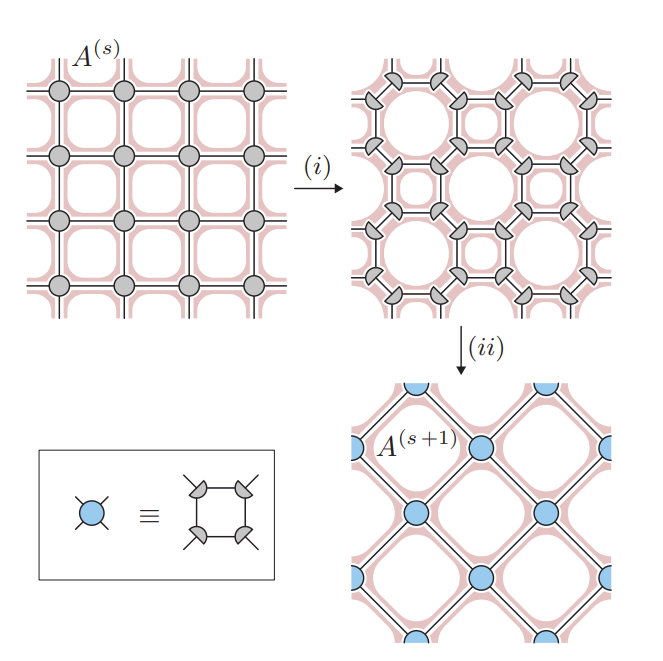
\includegraphics[width=0.8 \textwidth]{Figuren/tnalgs/TRG.png}
    \caption{ Steps in TRG procedure. Figure taken from \cite{Hauru}.  }
    \label{fig:tnalgs:trg}
\end{figure}

The general idea behind these methods is to course grain the \Gls{TN}. The first  algorithm in this group of methods was Tensor Renormalisation Group (TRG)  \cite{Hauru}, shown in \cref{fig:tnalgs:trg}. In the first step $(i)$, the tensors are split with an \Gls{SVD} in 2 different ways, depending on the position on the lattice. Step $(ii)$ recombines 4 halves of the decomposition into 1 new tensor. The result is a rotated grid, with side length $\sqrt{2}$. The bond dimension is truncated during the \Gls{SVD} step.
Many other variants exist, such as Tensor Network Renormalisation (TNR), which will not be discussed here.

\subsubsection{Corner Transfer Matrix methods}

\begin{figure}[!htbp]
    \centering
    \begin{subfigure}[b]{0.8\textwidth}
        \centering
        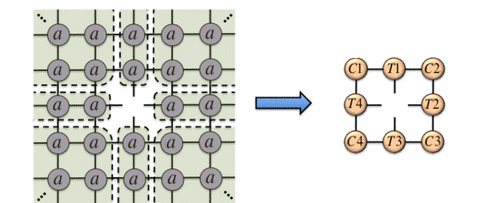
\includegraphics[width=\textwidth]{Figuren/tnalgs/CTMRG_Def.png   }
        \caption{Definition of environment}
        \label{fig:tnalgs:ctmrg:a}
    \end{subfigure}

    \begin{subfigure}[b]{0.7\textwidth}
        \centering
        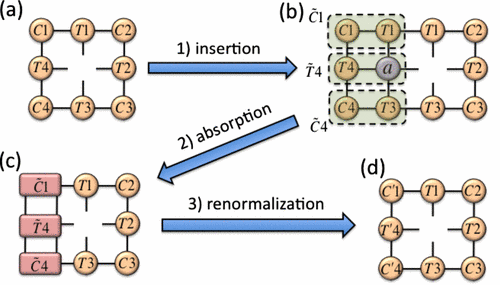
\includegraphics[width=\textwidth]{Figuren/tnalgs/CTMRG.png   }
        \caption{3 steps of CTMRG}
        \label{fig:tnalgs:ctmrg:b}
    \end{subfigure}
    \caption{  Figures adapted from \cite{orus} }
    \label{fig:tnalgs:ctmrg}
\end{figure}

\noindent
Another method goes by the name \Gls{CTMRG}, as described in \cite{orus}. The full network is approximated by 4 corner matrices C and 4 half row transfer matrices T as shown in \cref{fig:tnalgs:ctmrg:a}. The idea is to find matrices such that inserting a row and truncating it again results in the same tensors. This is shown in \cref{fig:tnalgs:ctmrg:b}. First, a new row is inserted. From \cref{fig:tnalgs:ctmrg:a} it can be seen that this should not change the environment. Some tensors are taken together in step 2. As a final step, the tensors are suitably truncated. Once this cycle converges, the environment is known. Note that many important details are not written down here, and this is merely to give some intuition about \Gls{TN} contraction algorithms.

\subsubsection{Boundary methods}

The goal of these methods is to find an \Gls{MPS} fixed point for the infinite lattice:

\begin{equation}\label{algs:mpslayermpo}
    \pepob{5}{3}{{
                "-","-", "-","-",
                "","","","",
                "","","","",}}{{
                "-", "-",
                "", "",
                "", "",
                "", "",
                "-", "-",}}{{
                4,4,4,4,4,
                13,0,0,0,13,
                13,2,7,3,13}}  \approx  \pepob{5}{2}{{
                "-","-", "-","-",
                "","","",""}}{{
                "-",
                "",
                "",
                "",
                "-"}}{{
                4,4,4,4,4,
                13,2,7,3,13}}
\end{equation}

\paragraph{Time-evolving block decimation}

Time-evolving block decimation was introduced as a method to calculate thermal states (this will also be encountered later on in \cref{rt_tn_methods}). It can also be used as a power method for contraction. The boundary \Gls{MPS} is applied to the MPO, and afterwards the enlarged MPO is truncated. This is done between all the even and odd sites, and afterwards between all odd and even sites. When this procedure is applied enough times, a fixed point is reached.

% \todo{explain this}

% \begin{figure}[!htbp]
%     \center
%     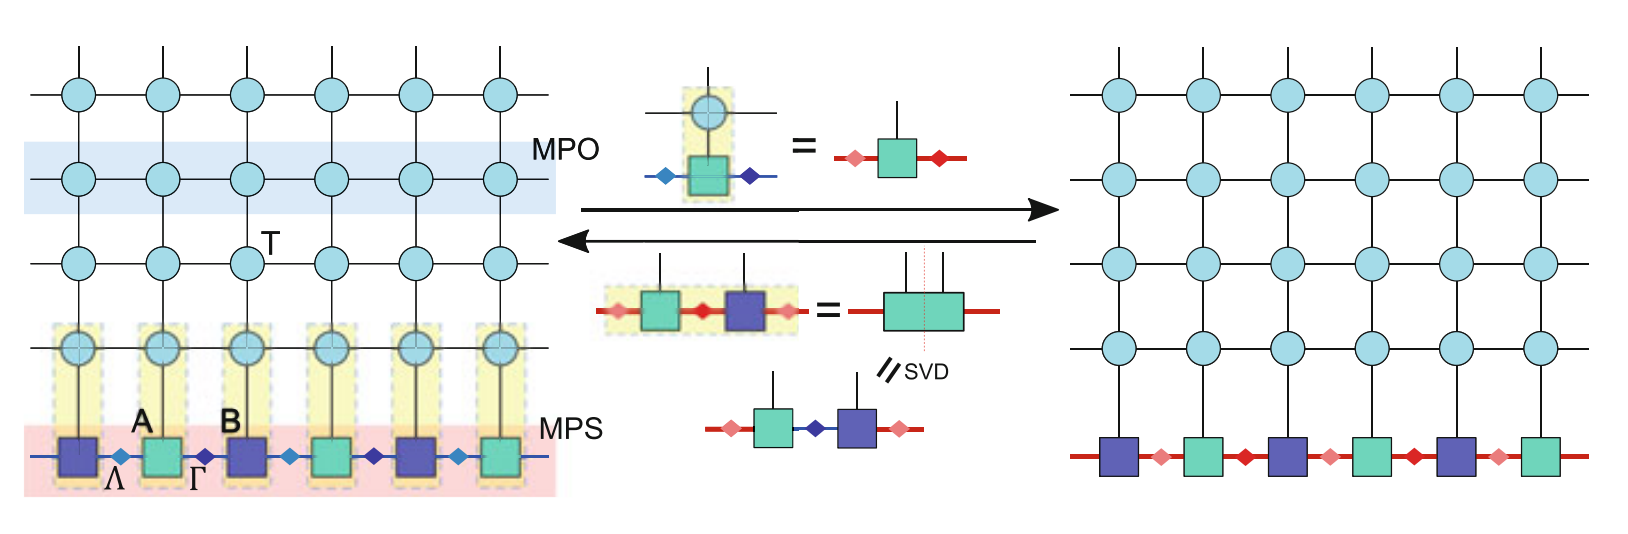
\includegraphics[width=1 \textwidth]{Figuren/tnalgs/tn_con_TEBD.png}
%     \caption{  Figure taken from \cite{Ran2020}.  }
%     \label{fig:tnalgs:tebd}
% \end{figure}

\subsection{VUMPS}

The purpose of this section is to give some intuition on the \Gls{VUMPS} algorithm, which will be used later on in this thesis. The goal is to find an \Gls{MPS} layer for the \Gls{MPO} (see \cref{algs:exp}). The expression holds approximately, because the \Gls{MPS} on the left-hand side has a larger bond dimension than on the right-hand side.

\subsubsection{The equations}
The method looks for tensors $Gl$ and $Gr$ which fulfil the conditions
\begin{subequations} \label{algs:vumpsenv}
    \begin{alignat}{2}
                                 & \vcenter{ \hbox{  \pepob{5}{3}{{
                            "","-", "-","",
                            "","Gl","","",
                            "","","",""}}{{
                            "-","-",
                            "-","-",
                            "","",
                            "-","-",
                            "",""}}{{
                            1,4,4,4,1,
                            1,4,0,4,1,
        1,5,2,4,1}} }} = \lambda &                                   & \vcenter{ \hbox{    \pepob{5}{3}{{
                            "-","-", "-","-",
                            "-","","Gl","-",
                            "-","","","-"}}{{
                            "-","-",
                            "-","-",
                            "","",
                            "-","-",
                            "-","-"}}{{
                            1,4,4,4,1,
                            1,4,2,4,1,
        1,1,5,4,1}}}}                                                                                     \\
                                 & \vcenter{ \hbox{   \pepob{5}{3}{{
                            "-","-", "-","-",
                            "","","Gr","-",
                            "","","",""}}{{
                            "-","-",
                            "-","-",
                            "","",
                            "-","-",
                            "-","-"}}{{
                            1,4,4,4,1,
                            1,4,0,4,1,
        1,4,8,1,1}} }}=  \lambda &                                   & \vcenter{ \hbox{ \pepob{5}{3}{{
                            "-","-", "-","-",
                            "-","-","Gr","",
                            "-","-","",""}}{{
                            "-","-",
                            "-","-",
                            "-","-",
                            "","",
                            "-","-"}}{{
                            1,1,4,4,4,
                            1,1,4,3,4,
                            1,1,10,1,1}} }} \;.
    \end{alignat}
\end{subequations}
These eigentensor equations are solved in practice in a slightly different manner
\begin{equation}\label{vumps_transfer_eigs}
    \vcenter{ \hbox{   \pepob{5}{3}{{
                        "-","", "","-",
                        "","","Gr","-",
                        "","","",""}}{{
                        "-","-",
                        "-","-",
                        "","",
                        "","",
                        "-","-"}}{{
                        1,4,3,4,1,
                        1,4,0,4,1,
                        1,4,8,1,1}} }}=  \lambda  \vcenter{ \hbox{ \pepob{5}{3}{{
                        "-","", "","",
                        "-","-","Gr","",
                        "-","-","",""}}{{
                        "-","-",
                        "-","-",
                        "-","-",
                        "","",
                        "",""}}{{
                        1,1,4,4,1,
                        1,1,4,4,1,
                        1,1,10,1,1}} }}\; ,
\end{equation}
where the $ Ar  $ tensor was connected from below on both sides and \cref{algs:mpsid} was used on the right-hand side. The blocks in \cref{algs:vumpsenv} form a zipper from the left and right respectively. Each application brings down one of the \Gls{MPS} tensors in the following way
\begin{equation}
    \begin{split}
        &       \vcenter{ \hbox{ \pepob{7}{3}{{
                            "-","-", "-","-","-","-",
                            "","Gl","","","","",
                            "","","","","","",}}{{
                            "-", "-",
                            "", "",
                            "", "",
                            "", "",
                            "", "",
                            "", "",
                            "-", "-",}}{{
                            1,4,4,4,4,4,4,
                            13,2,0,0,0,0,13,
                            1,5,2,2,2,2,13}}}} \\
        =&       \vcenter{ \hbox{ \pepob{7}{3}{{
                            "-","-", "-","-","-","-",
                            "","","Gl","","","",
                            "","","","","","",}}{{
                            "-", "-",
                            "", "",
                            "", "",
                            "", "",
                            "", "",
                            "", "",
                            "-", "-",}}{{
                            1,4,4,4,4,4,4,
                            13,2,2,0,0,0,13,
                            1,1,5,2,2,2,13}}}} \\
        =&       \vcenter{ \hbox{ \pepob{7}{3}{{
                            "-","-", "-","-","-","-",
                            "","","","Gl","","",
                            "","","","","","",}}{{
                            "-", "-",
                            "", "",
                            "", "",
                            "", "",
                            "", "",
                            "", "",
                            "-", "-",}}{{
                            1,4,4,4,4,4,4,
                            13,2,2,2,0,0,13,
                            1,1,1,5,2,2,13}}}} \; .
    \end{split}
\end{equation}
The left and right zipper can now move towards each other, until they meet at the center. One more condition is needed to fullfil \cref{algs:mpslayermpo}:
\begin{equation} \label{algs:AC}
    \vcenter{ \hbox{   \pepob{5}{3}{{
                        "-","-", "-","-",
                        "","Gl","Gr","-",
                        "","","",""}}{{
                        "-","-",
                        "-","-",
                        "","",
                        "-","-",
                        "-","-"}}{{
                        1,4,4,4,1,
                        1,4,0,4,1,
                        1,5,9,1,1}} }}=  \lambda_{AC} \; \pepob{3}{2}{{
                "-","-",
                "",""}}{{
                "-",
                "",
                "-"}}{{
                4,4,4,
                4,7,4}} \; .
\end{equation}
This completely determines the problem. One more equation is used in practice to solve the equations. Combining one of the equations in \ref{algs:vumpsenv}, the definition of $A_c$ \cref{algs:AC} and \cref{algs:mpsid} gives $C$
\begin{equation}\label{algs:vumpsenvc}
    \vcenter{ \hbox{   \pepob{5}{3}{{
                        "-","-", "-","-",
                        "","Gl","Gr","-",
                        "","","",""}}{{
                        "-","-",
                        "-","-",
                        "-","-",
                        "-","-",
                        "-","-"}}{{
                        1,4,4,4,1,
                        1,4,4,4,1,
                        1,5,11,1,1}} }}  =  \lambda_C \;  \pepob{3}{2}{{
                "-","-",
                "",""}}{{
                "-",
                "-",
                "-"}}{{
                4,4,4,
                4,6,4}}.
\end{equation}
Then  \cref{algs:mpslayermpo} is solved
\begin{equation}
    \begin{split}
        & \vcenter{ \hbox{ \pepob{7}{3}{{
                            "-","-", "-","-","-","-",
                            "","","","","","",
                            "","","","","","",}}{{
                            "-", "-",
                            "", "",
                            "", "",
                            "", "",
                            "", "",
                            "", "",
                            "-", "-",}}{{
                            4,4,4,4,4,4,4,
                            13,0,0,0,0,0,13,
                            13,2,2,7,3,3,13}} }}\\
        =&       \vcenter{ \hbox{ \pepob{7}{3}{{
                            "-","-", "-","-","-","-",
                            "","Gl","","","Gr","",
                            "","","","","","",}}{{
                            "-", "-",
                            "", "",
                            "", "",
                            "", "",
                            "", "",
                            "", "",
                            "-", "-",}}{{
                            1,4,4,4,4,4,4,
                            13,2,0,0,0,3,13,
                            1,5,2,7,8,1,4}}}} \\
        =&  \vcenter{ \hbox{ \pepob{7}{3}{{
                            "-","-", "-","-","-","-",
                            "","","Gl","Gr","","",
                            "","","","","","",}}{{
                            "-", "-",
                            "", "",
                            "", "",
                            "", "",
                            "", "",
                            "", "",
                            "-", "-",}}{{
                            1,4,4,4,4,4,4,
                            13,2,2,0,3,3,13,
                            1,1,5,9,1,1,1}} }}\\
        =& \vcenter{ \hbox{ \pepob{7}{3}{{
                            "-","-", "-","-","-","-",
                            "","","","","","",
                            "","","","","","",}}{{
                            "-", "-",
                            "", "",
                            "", "",
                            "", "",
                            "", "",
                            "", "",
                            "-", "-",}}{{
                            1,4,4,4,4,4,4,
                            13,2,2,7,3,3,13,
                            1,1,1,1,1,1,1}} }}.
    \end{split}
\end{equation}
Contracting a 2D \Gls{TN} is thus reduced to solving the  \cref{algs:ACC}, \cref{algs:vumpsenv}, \cref{algs:AC} and \cref{algs:vumpsenvc} simultaneously. Inspection of the equations shows that the following cycle occurs:
\begin{itemize}
    \item  $A_c,C  \rightarrow A_l,A_r  $  \cref{algs:ACC}
    \item  $A_l,A_r  \rightarrow Gl,Gr  $ \cref{algs:vumpsenv}
    \item  $ Gl,Gr   \rightarrow A_c,C $ \cref{algs:AC} and  \cref{algs:vumpsenvc}
\end{itemize}
The calculated environment (i.e\ the tensor $GL$,$Gr$ and \Gls{MPS} A) can now be used to solve the original problem. The same \Gls{MPS}  \footnote{this will not be always the case, see \cref{subsec:vumps_below_alt} } is applied to contract the \Gls{TN} from below. \Cref{algs:biggrid} now becomes
\begin{equation}\label{vumps_Below}
    \vcenter{ \hbox{   \pepob{5}{3}{{
                        "","", "","",
                        "","Gl","Gr","",
                        "","","",""}}{{
                        "-","-",
                        "","",
                        "","",
                        "","",
                        "-","-"}}{{
                        13,2,7,3,13,
                        13,2,12,3,13,
                        1,5,9,1,1}} }}.
\end{equation}
As always, the identity \eqref{algs:mpsid} can be used to simplify the equation to
\begin{equation}
    \vcenter{ \hbox{   \pepob{5}{3}{{
                        "","", "","",
                        "","Gl","Gr","",
                        "","","",""}}{{
                        "-","-",
                        "","",
                        "","",
                        "","",
                        "-","-"}}{{
                        1,4,7,4,1,
                        1,4,12,4,1,
                        1,5,9,1,1}} }}.
\end{equation}

\subsubsection{The derivation}\label{vumps_Deriv}
While the above derivation is reasonable, it is not very rigorous. The algorithm finds its origins  in tangent space methods, as explained in \cite{Vanderstraeten2019}. Not every state in the many body Hilbert space can be represented by an \Gls{MPS}. By carefully constructing the tangent space and making use of the available gauge freedom, a compact expression can be found for the tangent space projector $\mathcal{P}_A$. This projects a state from the many body Hilbert space onto the tangent space of an \Gls{MPS} A. For an optimal MPS approximation A, the error made in the approximation should be orthogonal to the tangent space. For \cref{algs:mpslayermpo} this means that the application of the projection of the error on the tangent space should be zero, i.e. the \Gls{MPS} is at a variational minimum   \cite{Nietner2020}. Applying the projector $\mathcal{P}_A$ to \cref{algs:mpslayermpo} exactly gives rise to the equations stated earlier.

\subsubsection{Multisite}
In \cite{Nietner2020}, a version of \Gls{VUMPS} is proposed that can compute the environment of an m by n unit cell with only a linear increase in computation cost. Larger unit cells might be needed for ground states with a non-trivial unit cell.

\subsubsection{Calculating the MPS from below}\label{subsec:vumps_below_alt}

One question, which does not seem to be answered in literature, is which tensor $B$ to use to complete the contraction from below for a complete general \Gls{MPO}
\begin{equation}
    \vcenter{ \hbox{   \pepob{5}{3}{{
                        "","", "","",
                        "","Gl","Gr","",
                        "","","",""}}{{
                        "-","-",
                        "","",
                        "","",
                        "","",
                        "-","-"}}{{
                        1,4,16,4,1,
                        1,4,12,4,1,
                        1,5, 9  ,1,1}} }} .
\end{equation}
We will get back to this question in \cref{subsec:results:loops_and_ext}. A method suggested to me, and used throughout this thesis, is finding the largest eigenvalue from below (similar to \cref{algs:AC}):
\begin{equation}
    \vcenter{ \hbox{   \pepob{5}{3}{{
                        "","", "","",
                        "","Gl","Gr","",
                        "","","",""}}{{
                        "-","-",
                        "","",
                        "","",
                        "","",
                        "-","-"}}{{
                        1,4,16,4,1,
                        1,4,0,4,1,
                        1,5, 18  ,1,1}} }}  = \lambda_B   \vcenter{ \hbox{  \pepob{3}{2}{{
                        "","",
                        "-","-"}}{{
                        "-",
                        "",
                        "-"}}{{
                        4,16,4,
                        4,4,4}} }}
\end{equation}
This has some problems: $B$ can not be brought into a canonical form according to \cref{algs:ACC} (in combination with the analogue of \cref{algs:vumpsenvc}), and hence does not represent a fixed point \Gls{MPS} as was the case from above. This also doesn't work in the multisite setting. This finding is not completely surprising, suppose we have a fixed point \Gls{MPS} $B$ (denoted by bold tensors) from below (for instance obtained by performing the \Gls{VUMPS} algorithm on an \Gls{MPO} rotated by 180 degrees), then contracting the upper half plane and the lower half plane amounts to:

\begin{equation}
    \vcenter{ \hbox{   \pepob{5}{3}{{
                        "","", "","",
                        "","Gl","Gr","",
                        "","","",""}}{{
                        "-","-",
                        "","",
                        "","",
                        "","",
                        "-","-"}}{{
                        13,22,25,23,13,
                        13,2,12,3,13,
                        1,5,9,1,1}} }}
\end{equation}
To solve this equation, the left and the right fixed points need to be calculated
\begin{equation}\label{eq:vumps_B_own}
    \vcenter{ \hbox{   \pepob{3}{2}{{
                        "","",
                        "",""}}{{
                        "",
                        "",
                        "-"}}{{
                        24, 22 ,4,
                        4,  2 ,4}} }} = \lambda_f    \vcenter{ \hbox{  \pepob{3}{2}{{
                        "","",
                        "",""}}{{
                        "",
                        "-",
                        "-"}}{{
                        24, 4 ,1,
                        4,  4 ,1}} }}
\end{equation}
Then (with $Fr$ the analogous fixed point from the right side) the problem becomes:
\begin{equation}
    \vcenter{ \hbox{   \pepob{5}{3}{{
                        "","", "","",
                        "","Gl","Gr","",
                        "","","",""}}{{
                        "-","-",
                        "","",
                        "","",
                        "","",
                        "-","-"}}{{
                        1,24,25,26,1,
                        1,4,12,4,1,
                        1,5, 9  ,1,1}} }}
\end{equation}
Both methods could be equal, if the following holds (up to a constant factor)
\begin{equation}
    \vcenter{ \hbox{  \pepob{3}{2}{{
                        "","",
                        "-","-"}}{{
                        "-",
                        "",
                        "-"}}{{
                        4,16,4,
                        4,4,4}} }} =   \vcenter{ \hbox{   \pepob{5}{3}{{
                        "","", "","",
                        "","","","",
                        "","","",""}}{{
                        "-","-",
                        "","",
                        "","",
                        "","",
                        "-","-"}}{{
                        4,24,25,26,4,
                        1,1, 4,1,1,
                        1,1, 1  ,1,1}} }}.
\end{equation}
Some numerical investigation is needed to test whether or not this method gives a correct result.

